
%% bare_conf.tex
%% V1.3
%% 2007/01/11
%% by Michael Shell
%% See:
%% http://www.michaelshell.org/
%% for current contact information.
%%
%% This is a skeleton file demonstrating the use of IEEEtran.cls
%% (requires IEEEtran.cls version 1.7 or later) with an IEEE conference paper.
%%
%% Support sites:
%% http://www.michaelshell.org/tex/ieeetran/
%% http://www.ctan.org/tex-archive/macros/latex/contrib/IEEEtran/
%% and
%% http://www.ieee.org/

%%*************************************************************************
%% Legal Notice:
%% This code is offered as-is without any warranty either expressed or
%% implied; without even the implied warranty of MERCHANTABILITY or
%% FITNESS FOR A PARTICULAR PURPOSE! 
%% User assumes all risk.
%% In no event shall IEEE or any contributor to this code be liable for
%% any damages or losses, including, but not limited to, incidental,
%% consequential, or any other damages, resulting from the use or misuse
%% of any information contained here.
%%
%% All comments are the opinions of their respective authors and are not
%% necessarily endorsed by the IEEE.
%%
%% This work is distributed under the LaTeX Project Public License (LPPL)
%% ( http://www.latex-project.org/ ) version 1.3, and may be freely used,
%% distributed and modified. A copy of the LPPL, version 1.3, is included
%% in the base LaTeX documentation of all distributions of LaTeX released
%% 2003/12/01 or later.
%% Retain all contribution notices and credits.
%% ** Modified files should be clearly indicated as such, including  **
%% ** renaming them and changing author support contact information. **
%%
%% File list of work: IEEEtran.cls, IEEEtran_HOWTO.pdf, bare_adv.tex,
%%                    bare_conf.tex, bare_jrnl.tex, bare_jrnl_compsoc.tex
%%*************************************************************************

% *** Authors should verify (and, if needed, correct) their LaTeX system  ***
% *** with the testflow diagnostic prior to trusting their LaTeX platform ***
% *** with production work. IEEE's font choices can trigger bugs that do  ***
% *** not appear when using other class files.                            ***
% The testflow support page is at:
% http://www.michaelshell.org/tex/testflow/



% Note that the a4paper option is mainly intended so that authors in
% countries using A4 can easily print to A4 and see how their papers will
% look in print - the typesetting of the document will not typically be
% affected with changes in paper size (but the bottom and side margins will).
% Use the testflow package mentioned above to verify correct handling of
% both paper sizes by the user's LaTeX system.
%
% Also note that the "draftcls" or "draftclsnofoot", not "draft", option
% should be used if it is desired that the figures are to be displayed in
% draft mode.
%
\documentclass[conference]{IEEEtran}

\usepackage{graphicx}
\usepackage{listings} % needed for the inclusion of source code
\usepackage{mips}
\usepackage[margin=0.5in]{geometry}

% the following is needed for syntax highlighting
\usepackage{color}

\definecolor{dkgreen}{rgb}{0,0.6,0}
\definecolor{gray}{rgb}{0.5,0.5,0.5}
\definecolor{mauve}{rgb}{0.58,0,0.82}

\lstset{ %
  language=[mips]Assembler,       % the language of the code
  basicstyle=\footnotesize,       % the size of the fonts that are used for the code
  numbers=left,                   % where to put the line-numbers
  numberstyle=\tiny\color{gray},  % the style that is used for the line-numbers
  stepnumber=1,                   % the step between two line-numbers. If it's 1, each line 
                                  % will be numbered
  numbersep=5pt,                  % how far the line-numbers are from the code
  backgroundcolor=\color{white},  % choose the background color. You must add \usepackage{color}
  showspaces=false,               % show spaces adding particular underscores
  showstringspaces=false,         % underline spaces within strings
  showtabs=false,                 % show tabs within strings adding particular underscores
  frame=single,                   % adds a frame around the code
  rulecolor=\color{black},        % if not set, the frame-color may be changed on line-breaks within not-black text (e.g. commens (green here))
  tabsize=4,                      % sets default tabsize to 2 spaces
  captionpos=b,                   % sets the caption-position to bottom
  breaklines=true,                % sets automatic line breaking
  breakatwhitespace=false,        % sets if automatic breaks should only happen at whitespace
  title=\lstname,                 % show the filename of files included with \lstinputlisting;
                                  % also try caption instead of title
  keywordstyle=\color{blue},          % keyword style
  commentstyle=\color{dkgreen},       % comment style
  stringstyle=\color{mauve},         % string literal style
  escapeinside={\%*}{*)},            % if you want to add a comment within your code
  morekeywords={*,...}               % if you want to add more keywords to the set
}

% Add the compsoc option for Computer Society conferences.
%
% If IEEEtran.cls has not been installed into the LaTeX system files,
% manually specify the path to it like:
% \documentclass[conference]{../sty/IEEEtran}





% Some very useful LaTeX packages include:
% (uncomment the ones you want to load)


% *** MISC UTILITY PACKAGES ***
%
%\usepackage{ifpdf}
% Heiko Oberdiek's ifpdf.sty is very useful if you need conditional
% compilation based on whether the output is pdf or dvi.
% usage:
% \ifpdf
%   % pdf code
% \else
%   % dvi code
% \fi
% The latest version of ifpdf.sty can be obtained from:
% http://www.ctan.org/tex-archive/macros/latex/contrib/oberdiek/
% Also, note that IEEEtran.cls V1.7 and later provides a builtin
% \ifCLASSINFOpdf conditional that works the same way.
% When switching from latex to pdflatex and vice-versa, the compiler may
% have to be run twice to clear warning/error messages.






% *** CITATION PACKAGES ***
%
%\usepackage{cite}
% cite.sty was written by Donald Arseneau
% V1.6 and later of IEEEtran pre-defines the format of the cite.sty package
% \cite{} output to follow that of IEEE. Loading the cite package will
% result in citation numbers being automatically sorted and properly
% "compressed/ranged". e.g., [1], [9], [2], [7], [5], [6] without using
% cite.sty will become [1], [2], [5]--[7], [9] using cite.sty. cite.sty's
% \cite will automatically add leading space, if needed. Use cite.sty's
% noadjust option (cite.sty V3.8 and later) if you want to turn this off.
% cite.sty is already installed on most LaTeX systems. Be sure and use
% version 4.0 (2003-05-27) and later if using hyperref.sty. cite.sty does
% not currently provide for hyperlinked citations.
% The latest version can be obtained at:
% http://www.ctan.org/tex-archive/macros/latex/contrib/cite/
% The documentation is contained in the cite.sty file itself.






% *** GRAPHICS RELATED PACKAGES ***
%
\ifCLASSINFOpdf
  % \usepackage[pdftex]{graphicx}
  % declare the path(s) where your graphic files are
  % \graphicspath{{../pdf/}{../jpeg/}}
  % and their extensions so you won't have to specify these with
  % every instance of \includegraphics
  % \DeclareGraphicsExtensions{.pdf,.jpeg,.png}
\else
  % or other class option (dvipsone, dvipdf, if not using dvips). graphicx
  % will default to the driver specified in the system graphics.cfg if no
  % driver is specified.
  % \usepackage[dvips]{graphicx}
  % declare the path(s) where your graphic files are
  % \graphicspath{{../eps/}}
  % and their extensions so you won't have to specify these with
  % every instance of \includegraphics
  % \DeclareGraphicsExtensions{.eps}
\fi
% graphicx was written by David Carlisle and Sebastian Rahtz. It is
% required if you want graphics, photos, etc. graphicx.sty is already
% installed on most LaTeX systems. The latest version and documentation can
% be obtained at: 
% http://www.ctan.org/tex-archive/macros/latex/required/graphics/
% Another good source of documentation is "Using Imported Graphics in
% LaTeX2e" by Keith Reckdahl which can be found as epslatex.ps or
% epslatex.pdf at: http://www.ctan.org/tex-archive/info/
%
% latex, and pdflatex in dvi mode, support graphics in encapsulated
% postscript (.eps) format. pdflatex in pdf mode supports graphics
% in .pdf, .jpeg, .png and .mps (metapost) formats. Users should ensure
% that all non-photo figures use a vector format (.eps, .pdf, .mps) and
% not a bitmapped formats (.jpeg, .png). IEEE frowns on bitmapped formats
% which can result in "jaggedy"/blurry rendering of lines and letters as
% well as large increases in file sizes.
%
% You can find documentation about the pdfTeX application at:
% http://www.tug.org/applications/pdftex





% *** MATH PACKAGES ***
%
%\usepackage[cmex10]{amsmath}
% A popular package from the American Mathematical Society that provides
% many useful and powerful commands for dealing with mathematics. If using
% it, be sure to load this package with the cmex10 option to ensure that
% only type 1 fonts will utilized at all point sizes. Without this option,
% it is possible that some math symbols, particularly those within
% footnotes, will be rendered in bitmap form which will result in a
% document that can not be IEEE Xplore compliant!
%
% Also, note that the amsmath package sets \interdisplaylinepenalty to 10000
% thus preventing page breaks from occurring within multiline equations. Use:
%\interdisplaylinepenalty=2500
% after loading amsmath to restore such page breaks as IEEEtran.cls normally
% does. amsmath.sty is already installed on most LaTeX systems. The latest
% version and documentation can be obtained at:
% http://www.ctan.org/tex-archive/macros/latex/required/amslatex/math/





% *** SPECIALIZED LIST PACKAGES ***
%
%\usepackage{algorithmic}
% algorithmic.sty was written by Peter Williams and Rogerio Brito.
% This package provides an algorithmic environment fo describing algorithms.
% You can use the algorithmic environment in-text or within a figure
% environment to provide for a floating algorithm. Do NOT use the algorithm
% floating environment provided by algorithm.sty (by the same authors) or
% algorithm2e.sty (by Christophe Fiorio) as IEEE does not use dedicated
% algorithm float types and packages that provide these will not provide
% correct IEEE style captions. The latest version and documentation of
% algorithmic.sty can be obtained at:
% http://www.ctan.org/tex-archive/macros/latex/contrib/algorithms/
% There is also a support site at:
% http://algorithms.berlios.de/index.html
% Also of interest may be the (relatively newer and more customizable)
% algorithmicx.sty package by Szasz Janos:
% http://www.ctan.org/tex-archive/macros/latex/contrib/algorithmicx/




% *** ALIGNMENT PACKAGES ***
%
%\usepackage{array}
% Frank Mittelbach's and David Carlisle's array.sty patches and improves
% the standard LaTeX2e array and tabular environments to provide better
% appearance and additional user controls. As the default LaTeX2e table
% generation code is lacking to the point of almost being broken with
% respect to the quality of the end results, all users are strongly
% advised to use an enhanced (at the very least that provided by array.sty)
% set of table tools. array.sty is already installed on most systems. The
% latest version and documentation can be obtained at:
% http://www.ctan.org/tex-archive/macros/latex/required/tools/


%\usepackage{mdwmath}
%\usepackage{mdwtab}
% Also highly recommended is Mark Wooding's extremely powerful MDW tools,
% especially mdwmath.sty and mdwtab.sty which are used to format equations
% and tables, respectively. The MDWtools set is already installed on most
% LaTeX systems. The lastest version and documentation is available at:
% http://www.ctan.org/tex-archive/macros/latex/contrib/mdwtools/


% IEEEtran contains the IEEEeqnarray family of commands that can be used to
% generate multiline equations as well as matrices, tables, etc., of high
% quality.


%\usepackage{eqparbox}
% Also of notable interest is Scott Pakin's eqparbox package for creating
% (automatically sized) equal width boxes - aka "natural width parboxes".
% Available at:
% http://www.ctan.org/tex-archive/macros/latex/contrib/eqparbox/





% *** SUBFIGURE PACKAGES ***
%\usepackage[tight,footnotesize]{subfigure}
% subfigure.sty was written by Steven Douglas Cochran. This package makes it
% easy to put subfigures in your figures. e.g., "Figure 1a and 1b". For IEEE
% work, it is a good idea to load it with the tight package option to reduce
% the amount of white space around the subfigures. subfigure.sty is already
% installed on most LaTeX systems. The latest version and documentation can
% be obtained at:
% http://www.ctan.org/tex-archive/obsolete/macros/latex/contrib/subfigure/
% subfigure.sty has been superceeded by subfig.sty.



%\usepackage[caption=false]{caption}
%\usepackage[font=footnotesize]{subfig}
% subfig.sty, also written by Steven Douglas Cochran, is the modern
% replacement for subfigure.sty. However, subfig.sty requires and
% automatically loads Axel Sommerfeldt's caption.sty which will override
% IEEEtran.cls handling of captions and this will result in nonIEEE style
% figure/table captions. To prevent this problem, be sure and preload
% caption.sty with its "caption=false" package option. This is will preserve
% IEEEtran.cls handing of captions. Version 1.3 (2005/06/28) and later 
% (recommended due to many improvements over 1.2) of subfig.sty supports
% the caption=false option directly:
%\usepackage[caption=false,font=footnotesize]{subfig}
%
% The latest version and documentation can be obtained at:
% http://www.ctan.org/tex-archive/macros/latex/contrib/subfig/
% The latest version and documentation of caption.sty can be obtained at:
% http://www.ctan.org/tex-archive/macros/latex/contrib/caption/




% *** FLOAT PACKAGES ***
%
%\usepackage{fixltx2e}
% fixltx2e, the successor to the earlier fix2col.sty, was written by
% Frank Mittelbach and David Carlisle. This package corrects a few problems
% in the LaTeX2e kernel, the most notable of which is that in current
% LaTeX2e releases, the ordering of single and double column floats is not
% guaranteed to be preserved. Thus, an unpatched LaTeX2e can allow a
% single column figure to be placed prior to an earlier double column
% figure. The latest version and documentation can be found at:
% http://www.ctan.org/tex-archive/macros/latex/base/



%\usepackage{stfloats}
% stfloats.sty was written by Sigitas Tolusis. This package gives LaTeX2e
% the ability to do double column floats at the bottom of the page as well
% as the top. (e.g., "\begin{figure*}[!b]" is not normally possible in
% LaTeX2e). It also provides a command:
%\fnbelowfloat
% to enable the placement of footnotes below bottom floats (the standard
% LaTeX2e kernel puts them above bottom floats). This is an invasive package
% which rewrites many portions of the LaTeX2e float routines. It may not work
% with other packages that modify the LaTeX2e float routines. The latest
% version and documentation can be obtained at:
% http://www.ctan.org/tex-archive/macros/latex/contrib/sttools/
% Documentation is contained in the stfloats.sty comments as well as in the
% presfull.pdf file. Do not use the stfloats baselinefloat ability as IEEE
% does not allow \baselineskip to stretch. Authors submitting work to the
% IEEE should note that IEEE rarely uses double column equations and
% that authors should try to avoid such use. Do not be tempted to use the
% cuted.sty or midfloat.sty packages (also by Sigitas Tolusis) as IEEE does
% not format its papers in such ways.





% *** PDF, URL AND HYPERLINK PACKAGES ***
%
%\usepackage{url}
% url.sty was written by Donald Arseneau. It provides better support for
% handling and breaking URLs. url.sty is already installed on most LaTeX
% systems. The latest version can be obtained at:
% http://www.ctan.org/tex-archive/macros/latex/contrib/misc/
% Read the url.sty source comments for usage information. Basically,
% \url{my_url_here}.





% *** Do not adjust lengths that control margins, column widths, etc. ***
% *** Do not use packages that alter fonts (such as pslatex).         ***
% There should be no need to do such things with IEEEtran.cls V1.6 and later.
% (Unless specifically asked to do so by the journal or conference you plan
% to submit to, of course. )


% correct bad hyphenation here
%\hyphenation{op-tical net-works semi-conduc-tor}


\begin{document}
%
% paper title
% can use linebreaks \\ within to get better formatting as desired
\title{ECSE 548 (VLSI) Project: MIPS Processor On-Chip Cache Design and Integration}


% author names and affiliations
% use a multiple column layout for up to three different
% affiliations
%\author{\IEEEauthorblockN{Michael Shell}
%\IEEEauthorblockA{School of Electrical and\\Computer Engineering\\
%Georgia Institute of Technology\\
%Atlanta, Georgia 30332--0250\\
%Email: http://www.michaelshell.org/contact.html}
%\and
%\IEEEauthorblockN{Homer Simpson}
%\IEEEauthorblockA{Twentieth Century Fox\\
%Springfield, USA\\
%Email: homer@thesimpsons.com}
%\and
%\IEEEauthorblockN{James Kirk\\ and Montgomery Scott}
%\IEEEauthorblockA{Starfleet Academy\\
%San Francisco, California 96678-2391\\
%Telephone: (800) 555--1212\\
%Fax: (888) 555--1212}}

% conference papers do not typically use \thanks and this command
% is locked out in conference mode. If really needed, such as for
% the acknowledgment of grants, issue a \IEEEoverridecommandlockouts
% after \documentclass

% for over three affiliations, or if they all won't fit within the width
% of the page, use this alternative format:
% 
%\author{\IEEEauthorblockN{Michael Shell\IEEEauthorrefmark{1},
%Homer Simpson\IEEEauthorrefmark{2},
%James Kirk\IEEEauthorrefmark{3}, 
%Montgomery Scott\IEEEauthorrefmark{3} and
%Eldon Tyrell\IEEEauthorrefmark{4}}
%\IEEEauthorblockA{\IEEEauthorrefmark{1}School of Electrical and Computer Engineering\\
%Georgia Institute of Technology,
%Atlanta, Georgia 30332--0250\\ Email: see http://www.michaelshell.org/contact.html}
%\IEEEauthorblockA{\IEEEauthorrefmark{2}Twentieth Century Fox, Springfield, USA\\
%Email: homer@thesimpsons.com}
%\IEEEauthorblockA{\IEEEauthorrefmark{3}Starfleet Academy, San Francisco, California 96678-2391\\
%Telephone: (800) 555--1212, Fax: (888) 555--1212}
%\IEEEauthorblockA{\IEEEauthorrefmark{4}Tyrell Inc., 123 Replicant Street, Los Angeles, California 90210--4321}}




% use for special paper notices
%\IEEEspecialpapernotice{(Invited Paper)}




% make the title area
\maketitle


\begin{abstract}
%\boldmath
In this paper, we present an on-chip cache design and integration for 8-bit MIPS
processor. The cache that we adopt is a direct-mapped cache with 1 byte cache
blocks. It has a size of 16 bytes and is used for both instructions and data. We
apply a top-down design methodology, i.e. we start from the architecture level
and go down to its layout, with testings on each level. To integrate the cache,
	MIPS Finite State Machine (FSM) is modified accordingly, which results in
	controller architecture modifications. Assembly code is also rewritten to verify
	cache functionality. Design quality is tested using SPICE.
\end{abstract}
% IEEEtran.cls defaults to using nonbold math in the Abstract.
% This preserves the distinction between vectors and scalars. However,
% if the conference you are submitting to favors bold math in the abstract,
% then you can use LaTeX's standard command \boldmath at the very start
% of the abstract to achieve this. Many IEEE journals/conferences frown on
% math in the abstract anyway.

% no keywords




% For peer review papers, you can put extra information on the cover
% page as needed:
% \ifCLASSOPTIONpeerreview
% \begin{center} \bfseries EDICS Category: 3-BBND \end{center}
% \fi
%
% For peerreview papers, this IEEEtran command inserts a page break and
% creates the second title. It will be ignored for other modes.
\IEEEpeerreviewmaketitle



\section{Introduction}

Cache is a small memory that  contains the most recently accessed pieces of main memory, used to speed-up the processor-memory operation. Due to \textbf{Locality of Reference}, where a process at any given time accesses only a small region of memory, a cache helps significantly reduce processor I/O overhead by loading the small region that can be accessed by the processor with a much faster rate. For example, the typicall memory access time of 60 ns of a Pentium processor can be reduced to 15 ns with the presence of a cache \cite{intel}.

In this report, we propose a design for a simple direct-mapped cache for MIPS processor using SRAM memory bits. The report is divided into seven sections. Section \ref{cache_arch} and Section \ref{arch} provides detailed descriptions of propsed design for cache architecture and modifications on the existing MIPS processor for the integration between the two parts; then Section \ref{implementation} presents the process of implementing the design. In Sections \ref{testing} and \ref{quality}, both functional and performance testing on the design is discussed. Section \ref{conclusion} concludes the design process along with the whole report.

%
% no \IEEEPARstart
% You must have at least 2 lines in the paragraph with the drop letter
% (should never be an issue)


%\hfill mds
% 
%\hfill January 11, 2007

% An example of a floating figure using the graphicx package.
% Note that \label must occur AFTER (or within) \caption.
% For figures, \caption should occur after the \includegraphics.
% Note that IEEEtran v1.7 and later has special internal code that
% is designed to preserve the operation of \label within \caption
% even when the captionsoff option is in effect. However, because
% of issues like this, it may be the safest practice to put all your
% \label just after \caption rather than within \caption{}.
%
% Reminder: the "draftcls" or "draftclsnofoot", not "draft", class
% option should be used if it is desired that the figures are to be
% displayed while in draft mode.
%
%\begin{figure}[!t]
%\centering
%\includegraphics[width=2.5in]{myfigure}
% where an .eps filename suffix will be assumed under latex, 
% and a .pdf suffix will be assumed for pdflatex; or what has been declared
% via \DeclareGraphicsExtensions.
%\caption{Simulation Results}
%\label{fig_sim}
%\end{figure}

% Note that IEEE typically puts floats only at the top, even when this
% results in a large percentage of a column being occupied by floats.


% An example of a double column floating figure using two subfigures.
% (The subfig.sty package must be loaded for this to work.)
% The subfigure \label commands are set within each subfloat command, the
% \label for the overall figure must come after \caption.
% \hfil must be used as a separator to get equal spacing.
% The subfigure.sty package works much the same way, except \subfigure is
% used instead of \subfloat.
%
%\begin{figure*}[!t]
%\centerline{\subfloat[Case I]\includegraphics[width=2.5in]{subfigcase1}%
%\label{fig_first_case}}
%\hfil
%\subfloat[Case II]{\includegraphics[width=2.5in]{subfigcase2}%
%\label{fig_second_case}}}
%\caption{Simulation results}
%\label{fig_sim}
%\end{figure*}
%
% Note that often IEEE papers with subfigures do not employ subfigure
% captions (using the optional argument to \subfloat), but instead will
% reference/describe all of them (a), (b), etc., within the main caption.


% An example of a floating table. Note that, for IEEE style tables, the 
% \caption command should come BEFORE the table. Table text will default to
% \footnotesize as IEEE normally uses this smaller font for tables.
% The \label must come after \caption as always.
%
%\begin{table}[!t]
%% increase table row spacing, adjust to taste
%\renewcommand{\arraystretch}{1.3}
% if using array.sty, it might be a good idea to tweak the value of
% \extrarowheight as needed to properly center the text within the cells
%\caption{An Example of a Table}
%\label{table_example}
%\centering
%% Some packages, such as MDW tools, offer better commands for making tables
%% than the plain LaTeX2e tabular which is used here.
%\begin{tabular}{|c||c|}
%\hline
%One & Two\\
%\hline
%Three & Four\\
%\hline
%\end{tabular}
%\end{table}


% Note that IEEE does not put floats in the very first column - or typically
% anywhere on the first page for that matter. Also, in-text middle ("here")
% positioning is not used. Most IEEE journals/conferences use top floats
% exclusively. Note that, LaTeX2e, unlike IEEE journals/conferences, places
% footnotes above bottom floats. This can be corrected via the \fnbelowfloat
% command of the stfloats package.

\section{Cache Architecture}\label{cache_arch}
The MIPS processor presented in the course takes an 8-bit address line and 8-bit data line every time it reads data from external memory; to maintain a manageable project scale while ensuring basic functioanlity of the cache, the cache was designed to split up the address line into a 4-bit tag line and a 4-bit set line, where set signals are used for row selection in cache whereas tag signals are used for comparison to generate cache hits. The designed configuration results in a 16 8-bit data row in cache, making it capable of storing 16 bytes (4 distinctive assembly instructions) for MIPS.

The resulting design of the cache is shown in Figure \ref{fig:cache_arch}. Set signals are used to decode data rows inside SRAM arrays, and tag signals are used to compare the tags stored in cache to generate cache hit signals. Wite enable (\textit{we} as shown in figure) signal ensures the cache is writeable whenever it set to high. Additionally, for better stability, a validation bit (\textit{v}) was added to each row of SRAM array inside the cache to implement \textit{Compulsory Miss Strategy}, where the first read from cache is always guaranteed to generate a cache miss signal.

\begin{figure}[h!]
  \centering
    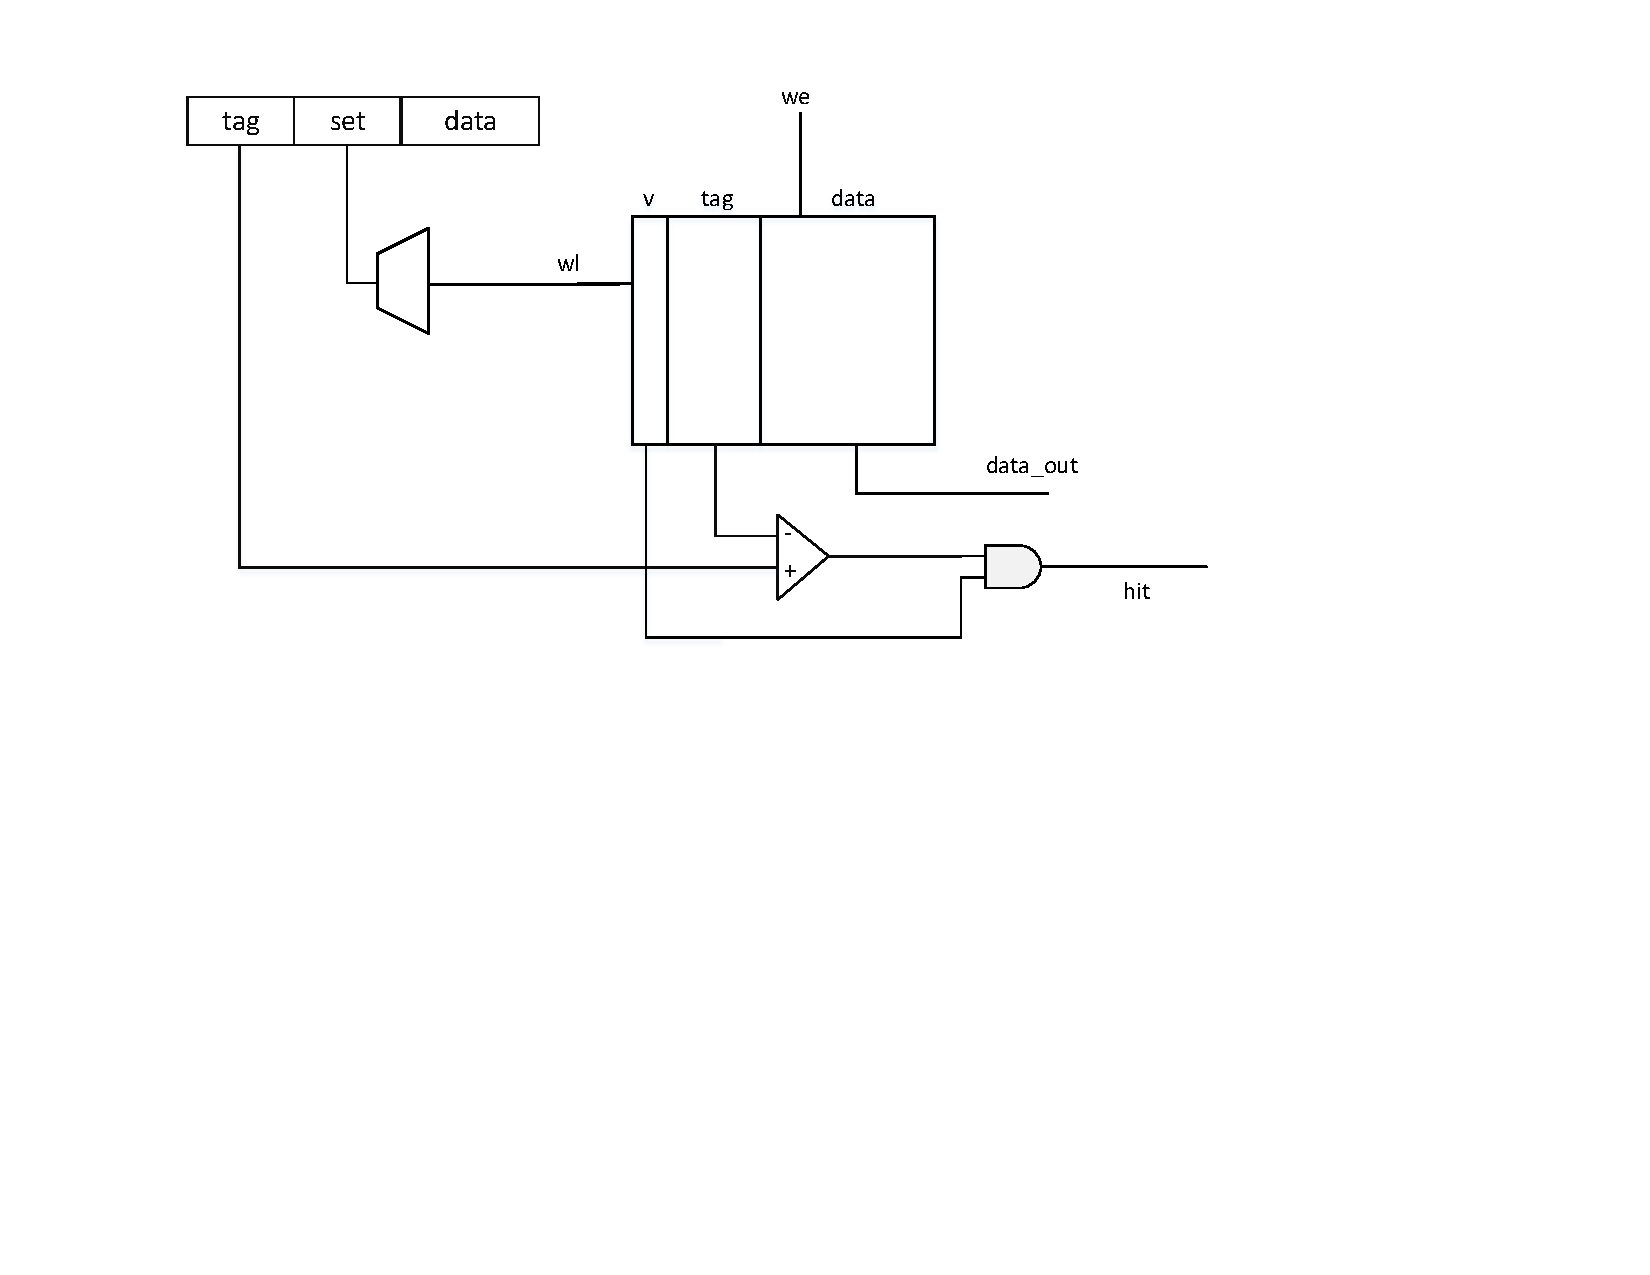
\includegraphics[width=0.45\textwidth]{cache_arch}
  \caption{Cache Microarchiture}
  \label{fig:cache_arch}
\end{figure}

\section{MIPS Integration Architecture}\label{arch}
We adopt hierarchical top-down design methodology. We go through architecture
level, schematic level and layout level. At architecture level, the Finite
State Machine (FSM) is modified and the controller is changed accordingly, see
Figure \ref{fig:fsm}. This is implemented in SystemVerilog and the functional simulation has
been verified successfully before going down to schematic level. The overall
MIPS microarchitecture is shown in Figure~\ref{fig:arch}.

\begin{figure}[h!]
  \centering
    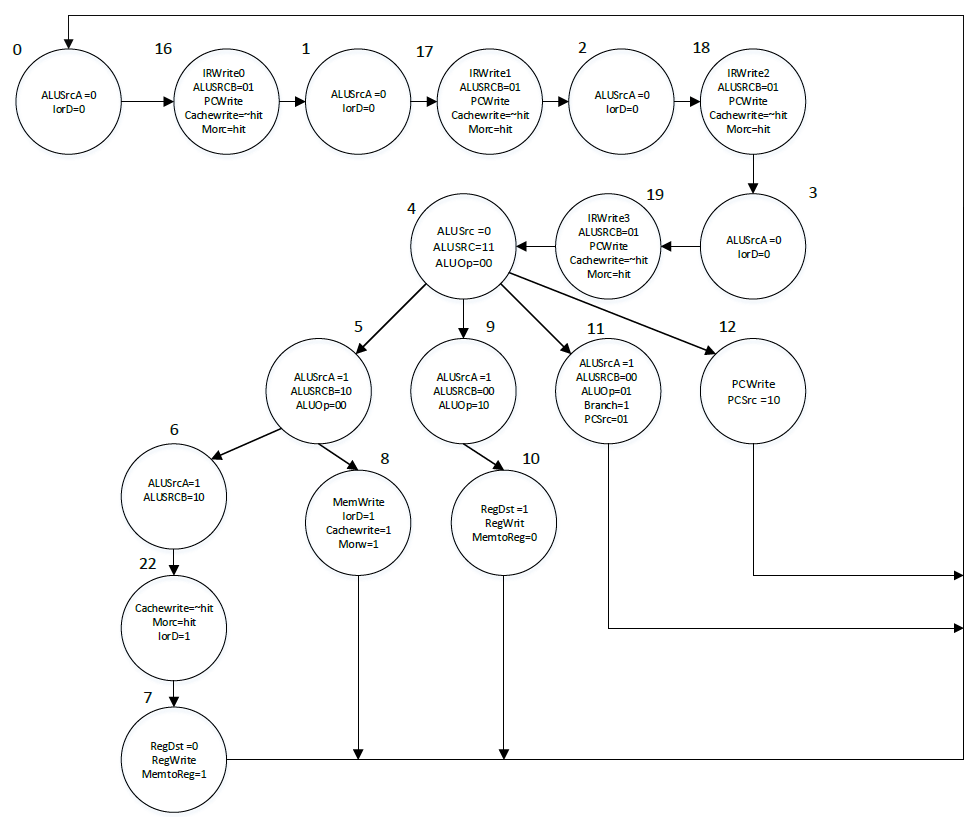
\includegraphics[width=0.55\textwidth]{fsm}
  \caption{Modified FSM of Controller}
  \label{fig:fsm}
\end{figure}

\begin{figure}[h!]
  \centering
    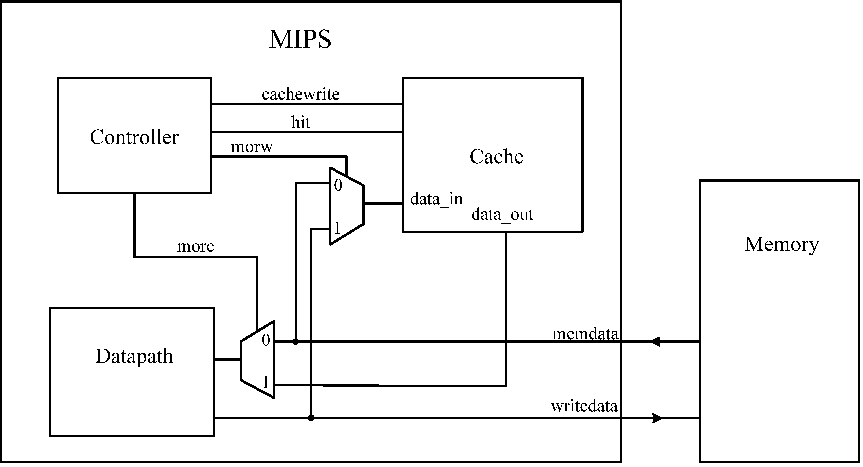
\includegraphics[width=0.4\textwidth]{arch.pdf}
  \caption{MIPS Microarchiture}
  \label{fig:arch}
\end{figure}


Since our cache is used for both instructions and data, in following sections,
	  when we say data, we refer to both instructions and data unless specified
	  otherwise. 

In Figure \ref{fig:arch}, three output signals (\textit{cachewrite, morw, morc}) and one input signal
(\textit{hit}) are added to the controller. 

\begin{itemize}
\item\textit{cachewrite} is used to
enable write/read access to the cache with a value of 1/0. 

\item\textit{morw} is used
to select data from memory or datapath. If a cache miss happens, it is set
to 0 and the data from memory is written into the cache. 

\item\textit{morc} is used to select data from memory or from cache. If there is a
cache hit, it is set to 1 and the data from cache is sent to MIPS. Otherwise it
is set to 0 and memory data is used.

\item\textit{hit} is used to show status of cache. 1 represents a cache hit and
0 represents a cache miss. A compulsory miss strategy was implemented for an ensured miss for a first-time read from cache.
\end{itemize}

In Figure \ref{fig:fsm}, we split one state for data read
access into two states. The first state is used to see if there is a cache hit.
If so, at second state, data from cache is read; otherwise data is fetched from
main memory. 

We adopt write-through policy, so the data is always written to both cache and
memory. For data write access, we still use one state.

\section{Implementaion}\label{implementation}
This section discusses the implementation process of cache components and integration in Electric.
\subsection{Comparator}\label{subsec:comparator}
A 4-bit comparator was implemented to compare the \textit{tag} bits from the memory and cache to generate corresponding \textit{cache hit} signals. The designed schematic and layout can be found in Figure \ref{fig:comparator}.
\begin{figure}[h!]
  \centering
    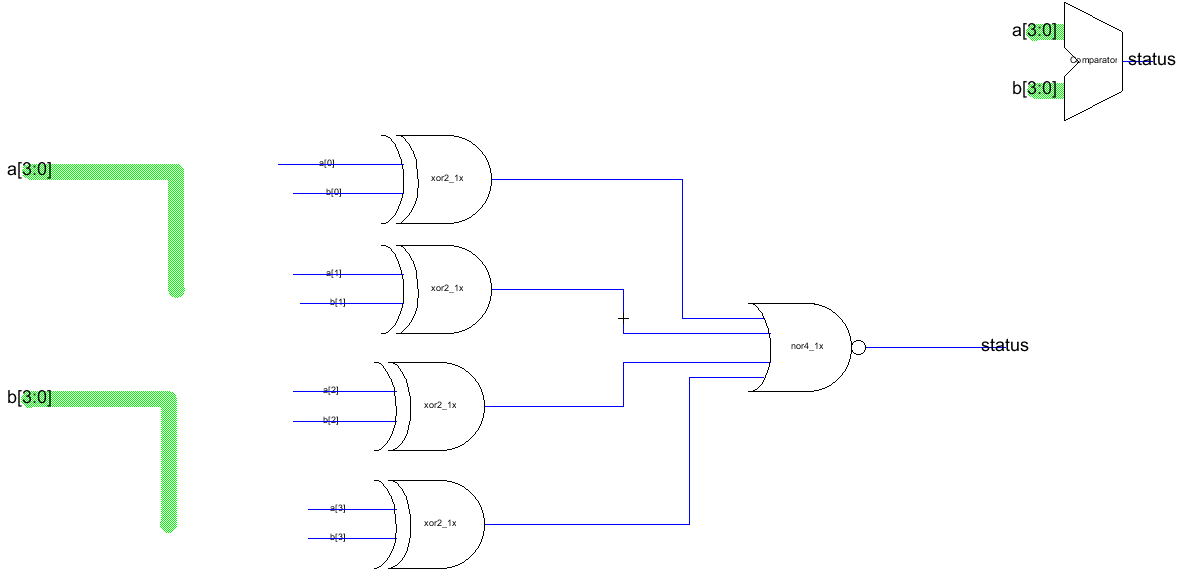
\includegraphics[width=0.25\textwidth]{comparator_sch} 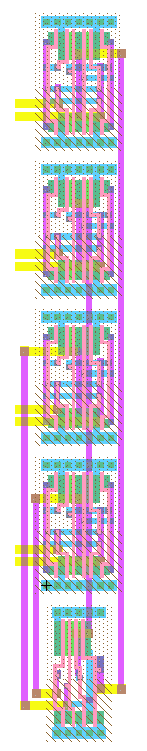
\includegraphics[scale=0.25]{comparator_layout}
  \caption{The Schematic and Layout of Comparator Design}
  \label{fig:comparator}
\end{figure}

Figure \ref{fig:comparator_check} indicates that the comparator design was valid, passing all three design rule checks.
\begin{figure}[h!]
  \centering
    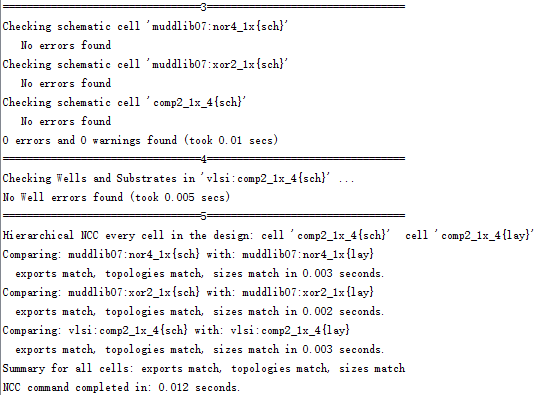
\includegraphics[width=0.4\textwidth]{comparator_check}
  \caption{Deisgn Rule Checks for Comparator}
  \label{fig:comparator_check}
\end{figure}

\subsection{4-to-16 Row Decoder}\label{subsec:decoder}
In order for the cache to make use of the 4-bit set signals, a row decoder was applied to decode the set signal and select 1 out of 16 8-bit data lines lying inside the cache. In order to reduce the delay and space usage of the decoder, \textit{pre-decoding} technology was used, resulting in a design shown in Figure \ref{fig:decoder}. It was worth noting that the layout of the decoder was delibrately designed to be wide with a minimum height in order to pitch-match with the sram array inside the cache.
\begin{figure}[h!]
  \centering
    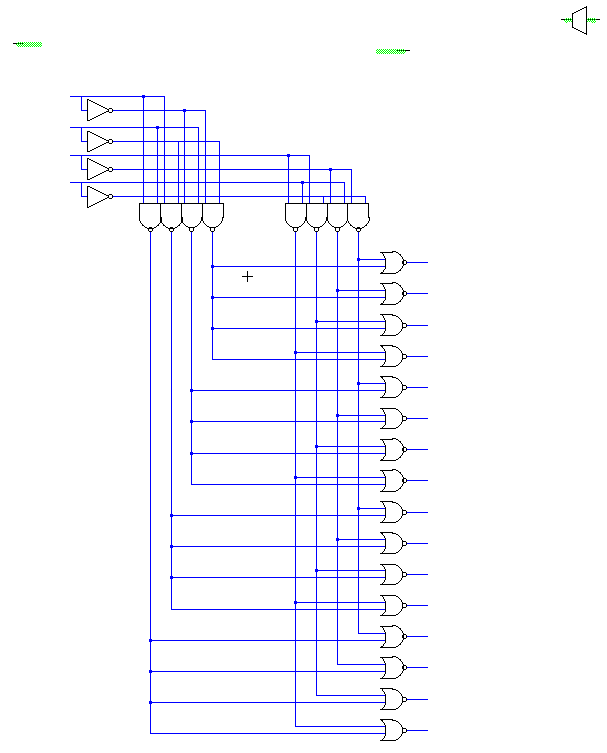
\includegraphics[width=0.15\textwidth]{decoder_sch} 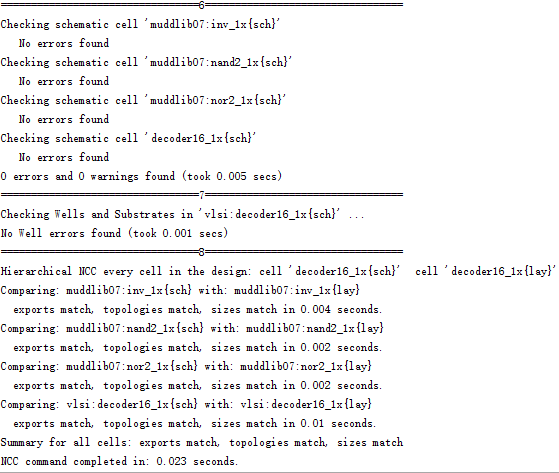
\includegraphics[width=0.3\textwidth]{decoder_check} 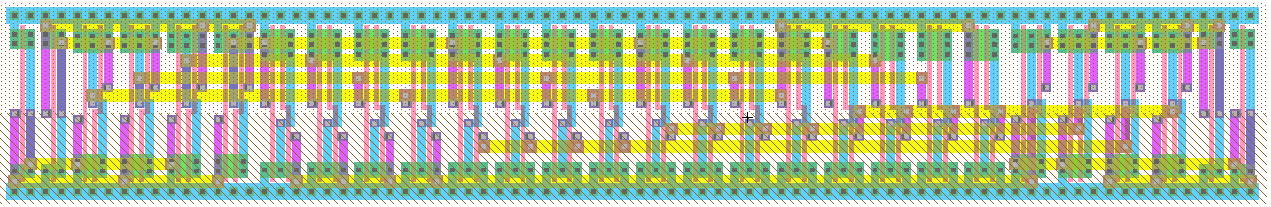
\includegraphics[scale=0.25]{decoder_lay}
  \caption{The Schematic and Layout of Decoder Design With Design Rule Check Results}
  \label{fig:decoder}
\end{figure}

It can be shown from the Figure \ref{fig:decoder} that the decoder design passed all three design rule checks and was ready for the integration into the cache deisgn.

\subsection{SRAM Column}\label{subsec:sram_col}
An SRAM column represents a column of SRAM bits inside the SRAM array of the cache, consisting of 16 SRAM bits sharing bit and inverting bit lines. The design was presented in Figure \ref{fig:sram_col}.

\begin{figure}[h!]
  \centering
    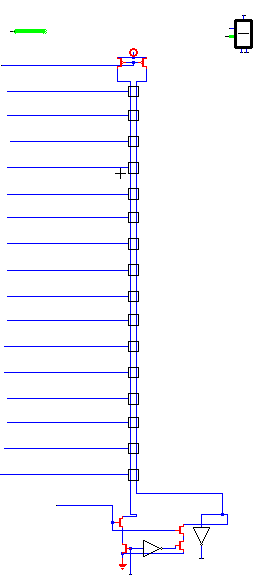
\includegraphics[width=0.15\textwidth]{sram_col_sch} 
\includegraphics[scale=0.3]{sram_col_lay} 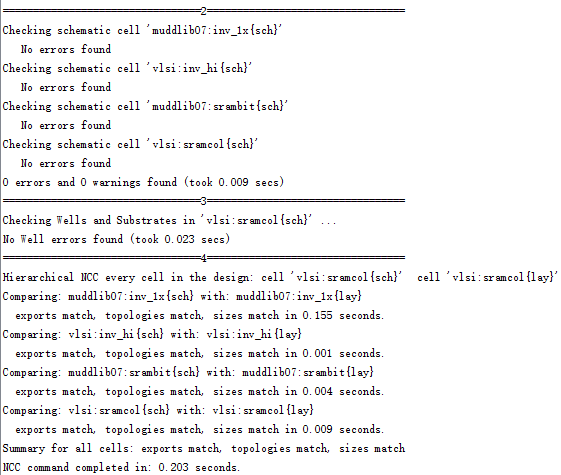
\includegraphics[width=0.3\textwidth]{sram_col_check}
  \caption{The Schematic and Layout of SRAM Column With Design Rule Check Results}
  \label{fig:sram_col}
\end{figure}

The design rule check results can be found in Figure \ref{fig:sram_col}. It can be shown from the Figure that all three of the design rule requirements were satisfied by the design.

\subsection{SRAM Array}\label{subsec:sram}
The SRAM array is the most essential part of the cache, consisting of 16 \textit{13-bit} SRAM bit rows, with each row having 1 bit for validation (compulsory miss), 4 bits for tag line and 8 bits for data storage. Each row also has a wordline buffer for a stable charging-up. The design is presented in Figure \ref{fig:sram}; the design rule check results can be found in the same figure as well.

\begin{figure}[h!]
  \centering
    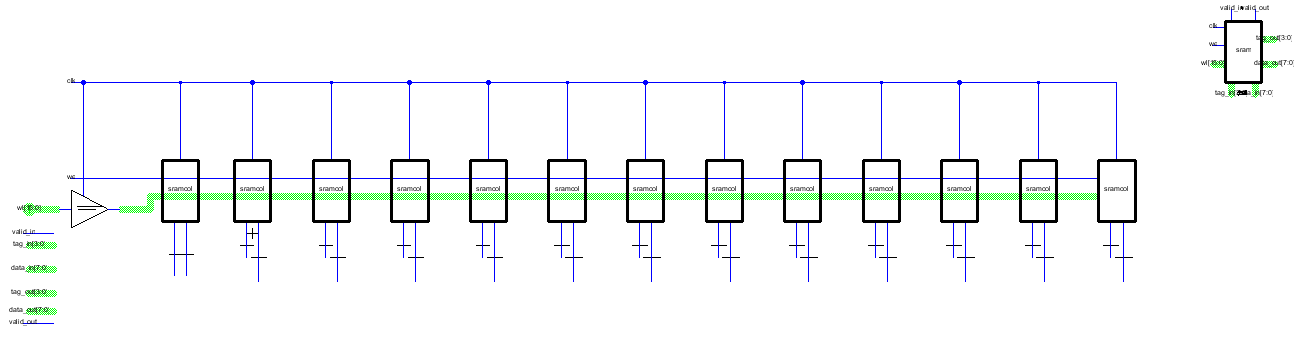
\includegraphics[width=0.4\textwidth]{sram_sch} 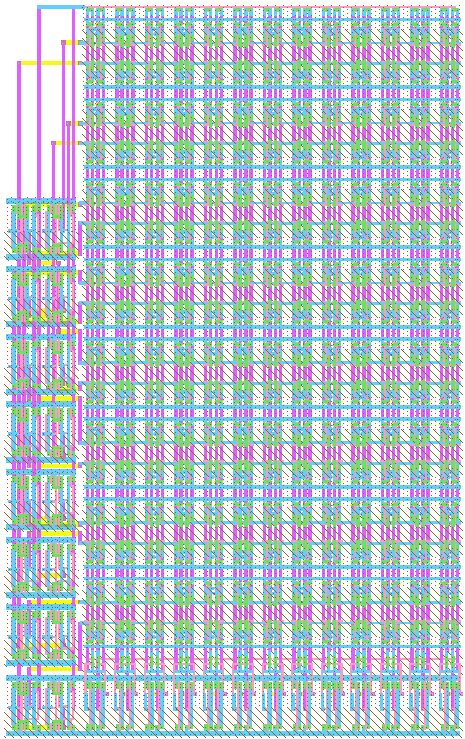
\includegraphics[scale=0.3]{sram_lay} 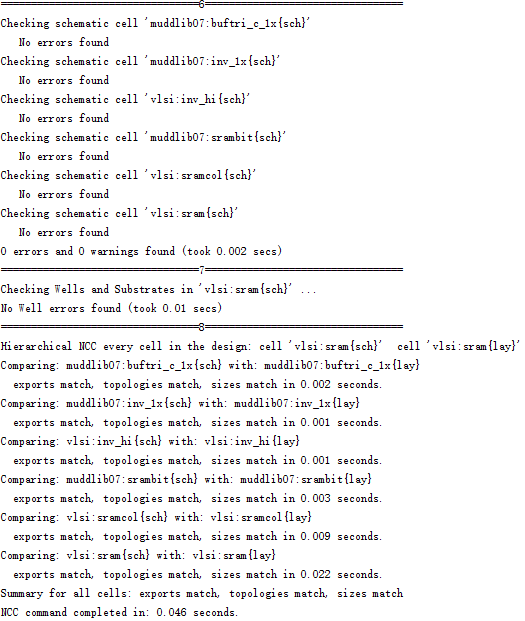
\includegraphics[width=0.25\textwidth]{sram_check}
  \caption{The Schematic and Layout of SRAM Array With Design Rule Check Results}
  \label{fig:sram}
\end{figure}

\subsection{Cache}\label{subsec:cache}
After the implementation of all circuit components, the cache was built based on the microarchitecture of the proposed cache circuit design. For easy integrations with the MIPS processor, in the layout, universal \textit{vdd} and \textit{gnd} tracks were added that connects \textit{vdd} and \textit{gnd} of sub-components together. The Cache circuit design, along with the evidence that it passes all three design checks, is presented in Figure \ref{fig:cache}.

\begin{figure}[h!]
  \centering
    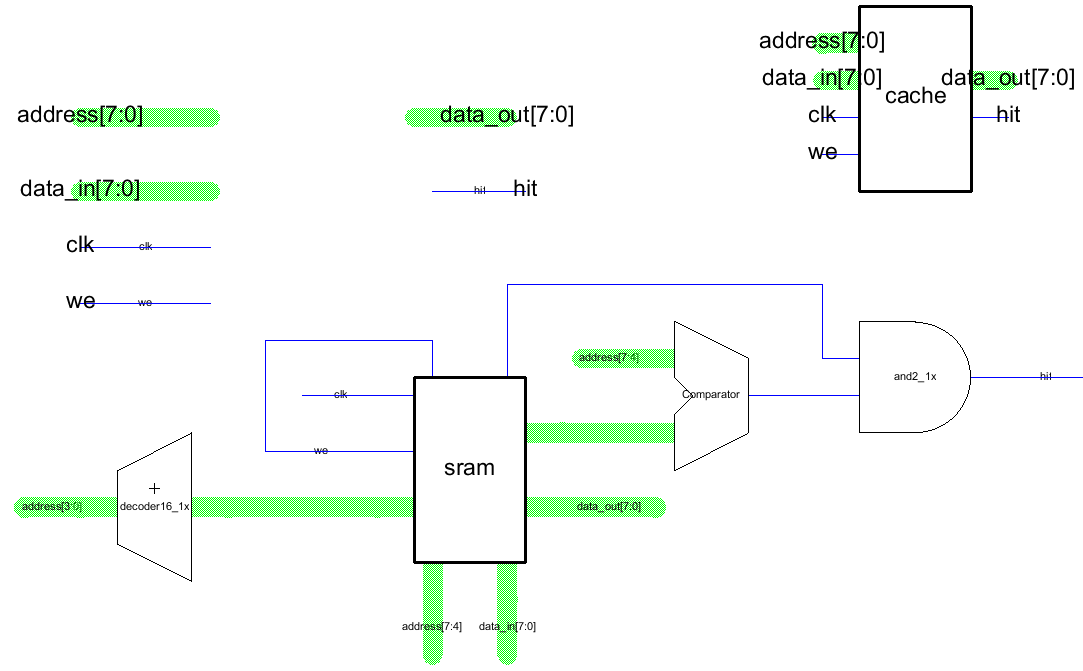
\includegraphics[width=0.3\textwidth]{cache_sch} 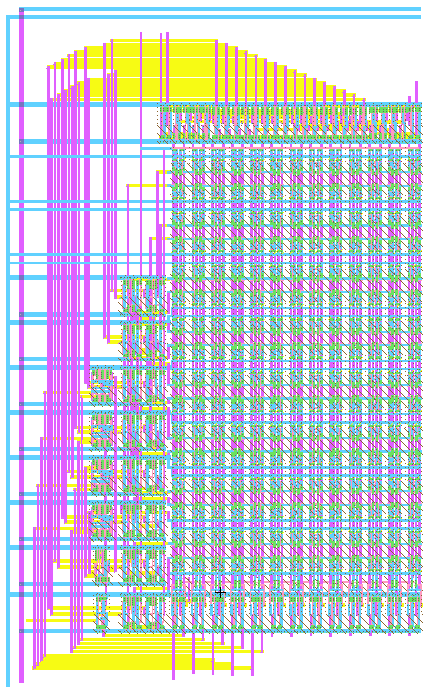
\includegraphics[scale=0.3]{cache_lay} 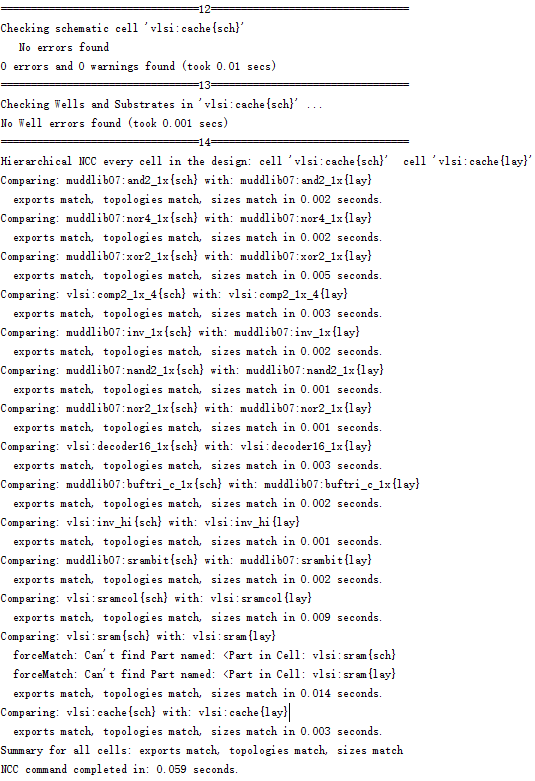
\includegraphics[width=0.25\textwidth]{cache_check}
  \caption{The Schematic and Layout of Cache With Design Rule Check Results}
  \label{fig:cache}
\end{figure}

\subsection{PLA Controller \& Controller}\label{subsec:controller}
As indicated in Section \ref{arch}, with updated FSM for the controller, the PLA controller which represents the FSM logic has been modified accordingly. With an updated FSM description file, a new PLA controller was generated and re-integrated into the controller citcuit of MIPS processor. New exports corresponding to cache signals have been added to the controller circtui as well. The resulting circuit is presented in the next sub-section.

\subsection{Integration}\label{subsec:integration}
Upon the completion and tests of each component, the cache was then integrated with MIPS processor (with updated controller component), resulting in a circuit presented in Figure \ref{fig:mips}.

\begin{figure}[h!]
  \centering
    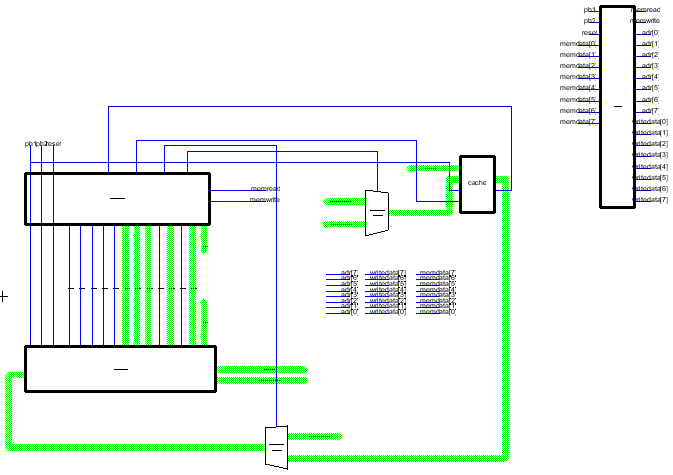
\includegraphics[width=0.3\textwidth]{mips_sch} 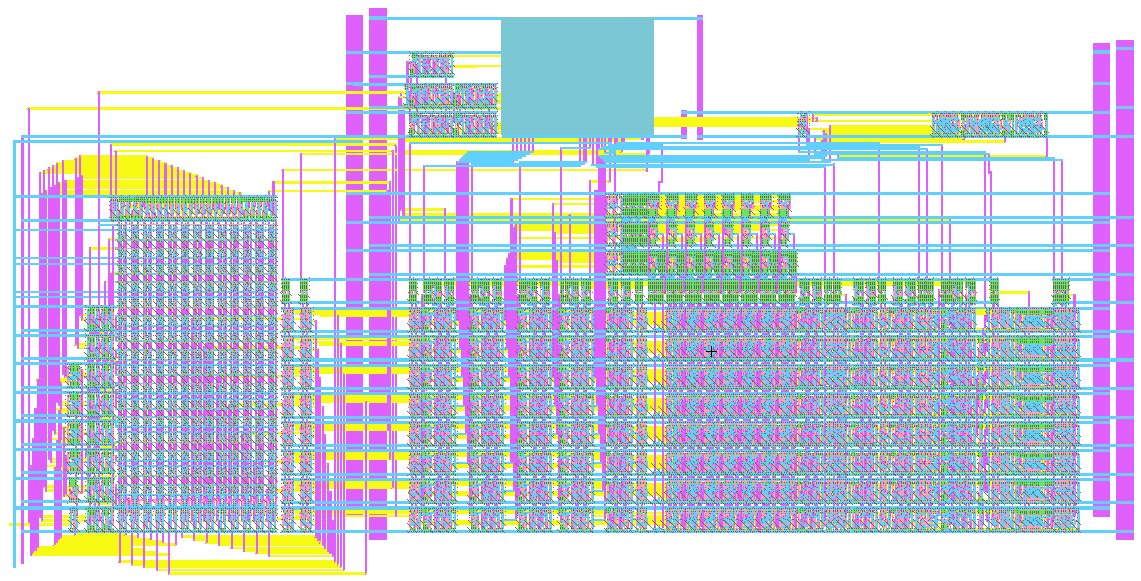
\includegraphics[scale=0.3]{mips_lay}
  \caption{The Schematic and Layout of MIPS integrated with Cache}
  \label{fig:mips}
\end{figure}

The pad frame was then generated from the new MIPS processor with cache implemented. To contain the much-expanded size of the MIPS, the size of the pad frame was extended from \textit{40} pads to \textit{64} pads. The resulting chip, along with error-free design rule check results, is shown in Figure \ref{fig:chip}. Due to page limits, a truncated version of design rule checks for the chip is presented in this report; the full check has been presented during the demo with the professor.

\begin{figure}[h!]
  \centering
    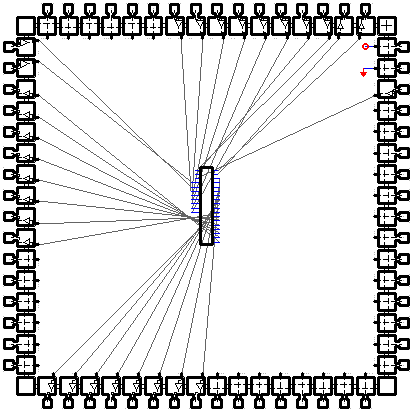
\includegraphics[width=0.2\textwidth]{chip_sch} 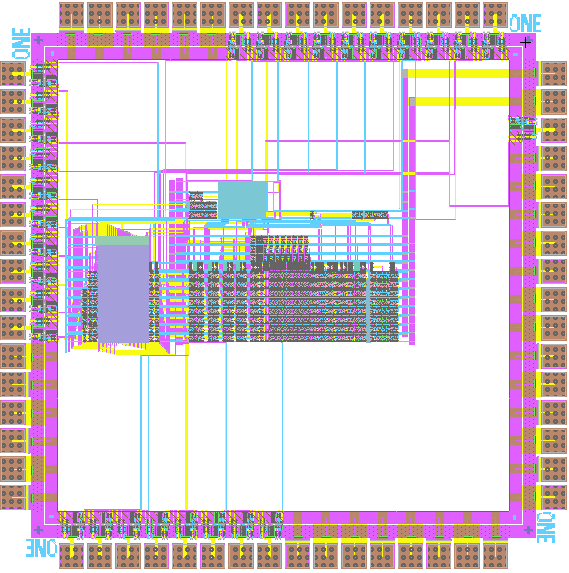
\includegraphics[scale=0.25]{chip_lay} 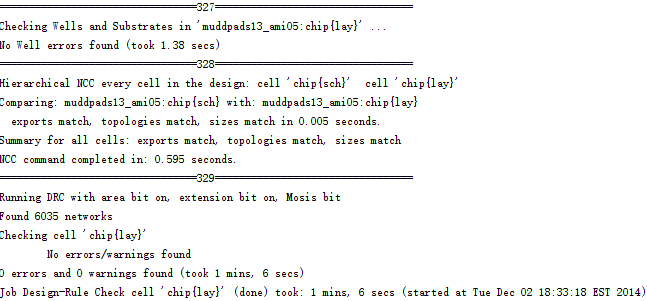
\includegraphics[width=0.3\textwidth]{chip_check}
  \caption{The Schematic and Layout of Chip Integration With Design Rule Check Results}
  \label{fig:chip}
\end{figure}

\section{Testing}\label{testing}
In this section, we explain our testing methodology. We tested components
individually in Section \ref{subsec:comp_test}. After assembly, the SystemVerilog MIPS
processor is simulated for functional testing in Section \ref{subsec:func_test}.

\subsection{Components Testing}\label{subsec:comp_test}
The main components to be tested are shown below:
\begin{itemize}
\item Comparator
\item Decoder
The 4-to-16 decoder was tested in ModelSim with all 16 test cases; the results showing that the design was operating properly is presented in Figure \ref{fig:decoder_test}.

\begin{figure}[h!]
  \centering
    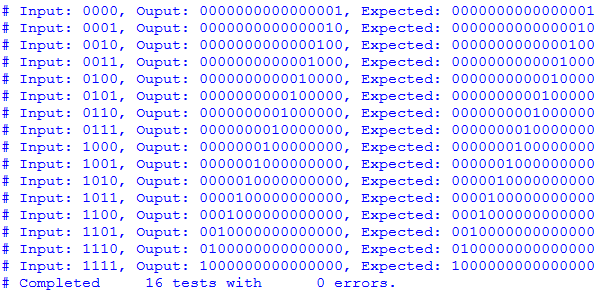
\includegraphics[width=0.3\textwidth]{decoder_test}
  \caption{ModelSim Test Results for decoder}
  \label{fig:decoder_test}
\end{figure}
 
\item SRAM: \\

This is the storage elements in cache. As shown in Figure \ref{fig:cache_arch}, it has 16 sets and each set consists of 1 \textit{valid} bit, 4 \textit{tag} bits and 8 \textit{data} bits. The input signal \textit{we} is set to 0/1 for data read/write and the signal \textit{wl} is used to select the set for access. Initially, the \textit{valid} bit is 0. Once a cache set is written, its corresponding \textit{valid} becomes 1. \textit{valid} is used to indicate if the data has been loaded or not. We produce some random inputs for testing. Due to the complexity of memory accesses, we generate test vectors from the inputs using our \textit{Python} script, as shown in Figure \ref{fig:sram_test}. The signal representation is listed in Table \ref{table:sram}. The functionality of SRAM is verified successfully according to test vectors.

\begin{figure}[h!]
  \centering
    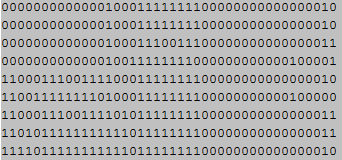
\includegraphics[width=0.3\textwidth]{sram_test.png}
  \caption{SRAM Test Vectors}
  \label{fig:sram_test}
\end{figure}

\begin{table}[h]
\centering
\caption{SRAM Test Vector}
\label{table:sram}
\begin{tabular}{c|c}
  \hline
  \textbf{bit position} & \textbf{signal}\\  
  \hline
  0 & we\\
  16:1 & wl \\
  24:17 & data\_in\\
  28:25 & tag\_in\\
  36:29 & expected\_data\\
  40:37 & expected\_tag\\
  41 & expected\_valid\\
  \hline
\end{tabular}
\end{table}

\end{itemize}

\subsection{Functional Testing}\label{subsec:func_test}
In this section, the functional testing of MIPS SystemVerilog model is
demonstrated. For this purpose, assembly code is written, as shown in Listing
\ref{lst:asm}.

\lstinputlisting[caption=Assembly Code, label=lst:asm]{test.s}
At the beginning, instructions are fetched, and there are compulsory cache misses. The assembly code contains a loop to test cache hits. When dealing with this loop, there are cache hits. In Figure \ref{fig:cache_miss}, we can see that there is a cache miss. This happens because the instructions are used for the first time here. During program execution, cache hits occur for the loop. This is illustrated in Figure \ref{fig:cache_hit}. The instructions in the loop are put in the cache and then fetched soon. As a result, cache hits happen here.

Apart from cache read access, we also checked cache write access, as shown in Figure \ref{fig:cache_write}. In this case, signal \textit{morw} is set to 1 to select data and \textit{cachewrite} is set to 1 to write the data from datapath into cache.

\begin{figure}[h!]
  \centering
    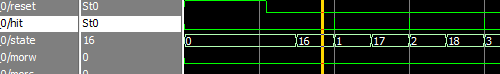
\includegraphics[width=0.3\textwidth]{cache_miss.png}
  \caption{Cache Read Miss}
  \label{fig:cache_miss}
\end{figure}

\begin{figure}[h!]
  \centering
    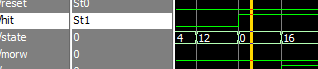
\includegraphics[width=0.3\textwidth]{cache_hit.png}
  \caption{Cache Read Hit}
  \label{fig:cache_hit}
\end{figure}

\begin{figure}[h!]
  \centering
    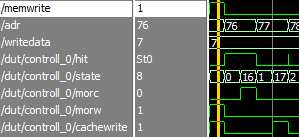
\includegraphics[width=0.3\textwidth]{cache_write.png}
  \caption{Cache Write}
  \label{fig:cache_write}
\end{figure}

The result is shown in Figure \ref{fig:cache_write}. If cache is absent, the write address \textit{adr} is 76 and write data \textit{writedata} is 7. After we integrated on-chip cache, the result is still correct. Our cache functionality is thus verified.

\section{Design Quality}\label{quality}
 
% power: and=> 1.89E-05  WATTS
%        inv=> 2.22E-05  WATTS
%		 hi-inv=>  1.27E-05  WATTS
 
 
In this section, performances of certain components, such as regular inverter, high-skew inverter as well as and gate, are evaluated using CAD tool(i.e.PSPICE) since we are not capable to perform evaluations directly on integrated circuits blocks due to the circuit size limitation from CAD tool. The corresponding results are shown in \textbf{Fig.\ref{fig:Spice}} for the setup time analysis of each component respectively. As can be seen clearly from the output waveform, the high-skew inverter pulls up faster than the regular inverter as expected. As for the power dissipation, the corresponding total power consumption of a and gate, inverter and high-skew inverter are $18.9\mu W$, $22.2\mu W$ and $12.7\mu W$, respectively. Therefore, skewed logic is clearly one of the high performance and low power-carry logic components available currently.

\begin{figure}[h!]
  \centering
    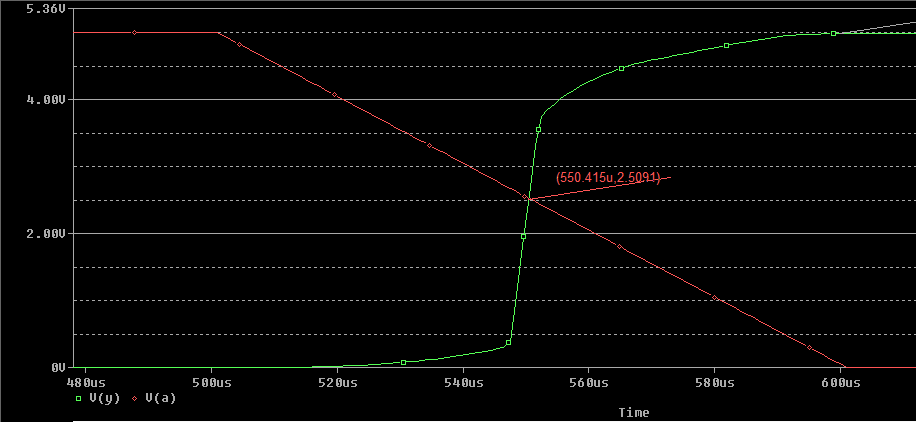
\includegraphics[width=0.23\textwidth]{inv} 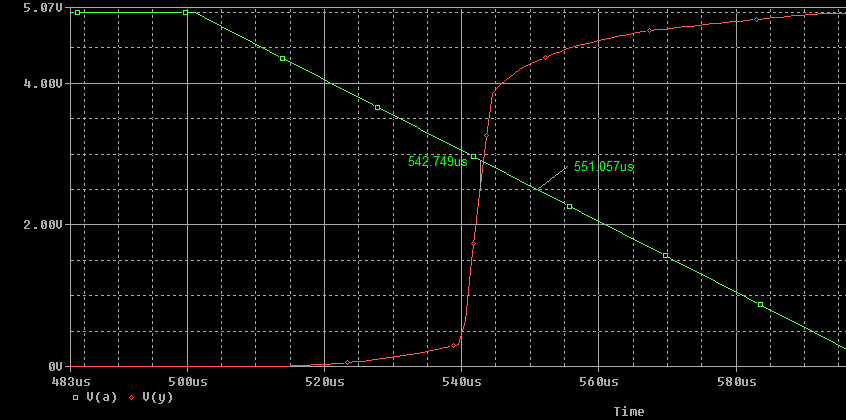
\includegraphics[scale=0.14]{hi} 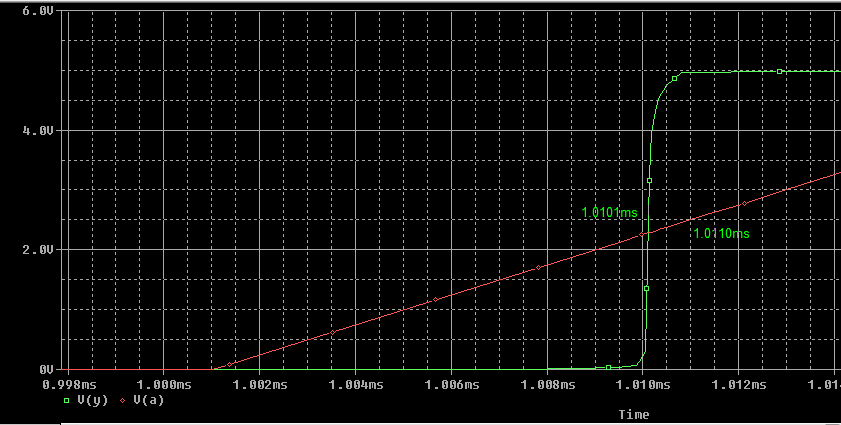
\includegraphics[width=0.3\textwidth]{and}
  \caption{SPICE simulation of INV, high-skew INV and AND gate}
  \label{fig:Spice}
\end{figure}

\section{Conclusion}\label{conclusion}

The Cache implementation can be mould in a number of ways, in terms of associativity which can decrease access time but increase complexity so in engineering world need to live with this trade-off. But basic working principal remains same.As discussed earlier we have successfully implemented the direct mapped cache and successful integration with MIPS.
cross severa the initially defined boundaries. It is important to understand that the
Pentium(R) Processor uses only one method to implement cache. We have successfully tested the all components their simulation verification done in ModelSim, Schematic and layout implementation and testing done in Electric. We also employed Spice simulation.In short Cache is simply a high speed memory that stores a piece of main memory which helps processor for high performance
he conclusion goes here.




% conference papers do not normally have an appendix


% use section* for acknowledgement
%\section*{Acknowledgment}
%
%
%The authors would like to thank...





% trigger a \newpage just before the given reference
% number - used to balance the columns on the last page
% adjust value as needed - may need to be readjusted if
% the document is modified later
%\IEEEtriggeratref{8}
% The "triggered" command can be changed if desired:
%\IEEEtriggercmd{\enlargethispage{-5in}}

% references section

% can use a bibliography generated by BibTeX as a .bbl file
% BibTeX documentation can be easily obtained at:
% http://www.ctan.org/tex-archive/biblio/bibtex/contrib/doc/
% The IEEEtran BibTeX style support page is at:
% http://www.michaelshell.org/tex/ieeetran/bibtex/
%\bibliographystyle{IEEEtran}
% argument is your BibTeX string definitions and bibliography database(s)
%\bibliography{IEEEabrv,../bib/paper}
%
% <OR> manually copy in the resultant .bbl file
% set second argument of \begin to the number of references
% (used to reserve space for the reference number labels box)
\begin{thebibliography}{1}

\bibitem{intel}http://download.intel.com/design/intarch/papers/cache6.pdf
The conclusion goes here.


\end{thebibliography}




% that's all folks
\end{document}


